\documentclass[a4j,titlepage]{jarticle}
\usepackage[dvipdfmx]{graphicx}
\usepackage{ascmac}
\usepackage{float}
\usepackage{amssymb}%にやりイコールを使う
\usepackage{multirow}
\usepackage{multicol}
%\usepackage{color}

\begin{document}

\title{2022 年度 3 回生前期学生実験 HW  \\ \bf team02 実施状況報告書}
% ↓ここに自分の氏名を記入
\author{実施状況報告書作成者:植田健斗\\
グループメンバー:\\伊藤舜一郎 (学籍番号:1029-32-7548)
\\植田健斗 (学籍番号:1029-32-6498)}
\西暦
\date{提出期限:5月12日18時 提出日: \today} % コンパイル時の日付が自動で挿入される
\maketitle
\newpage

\section{モジュール分割}

それぞれの機能を持った回路ごとにモジュール分割した。
各回路につけた名前は図\ref{moduleSplit0422}に示した通りである。(次の章の図\ref{rolesDivision0422}でまとめてある。)


\begin{figure}[H]
    \begin{center}
    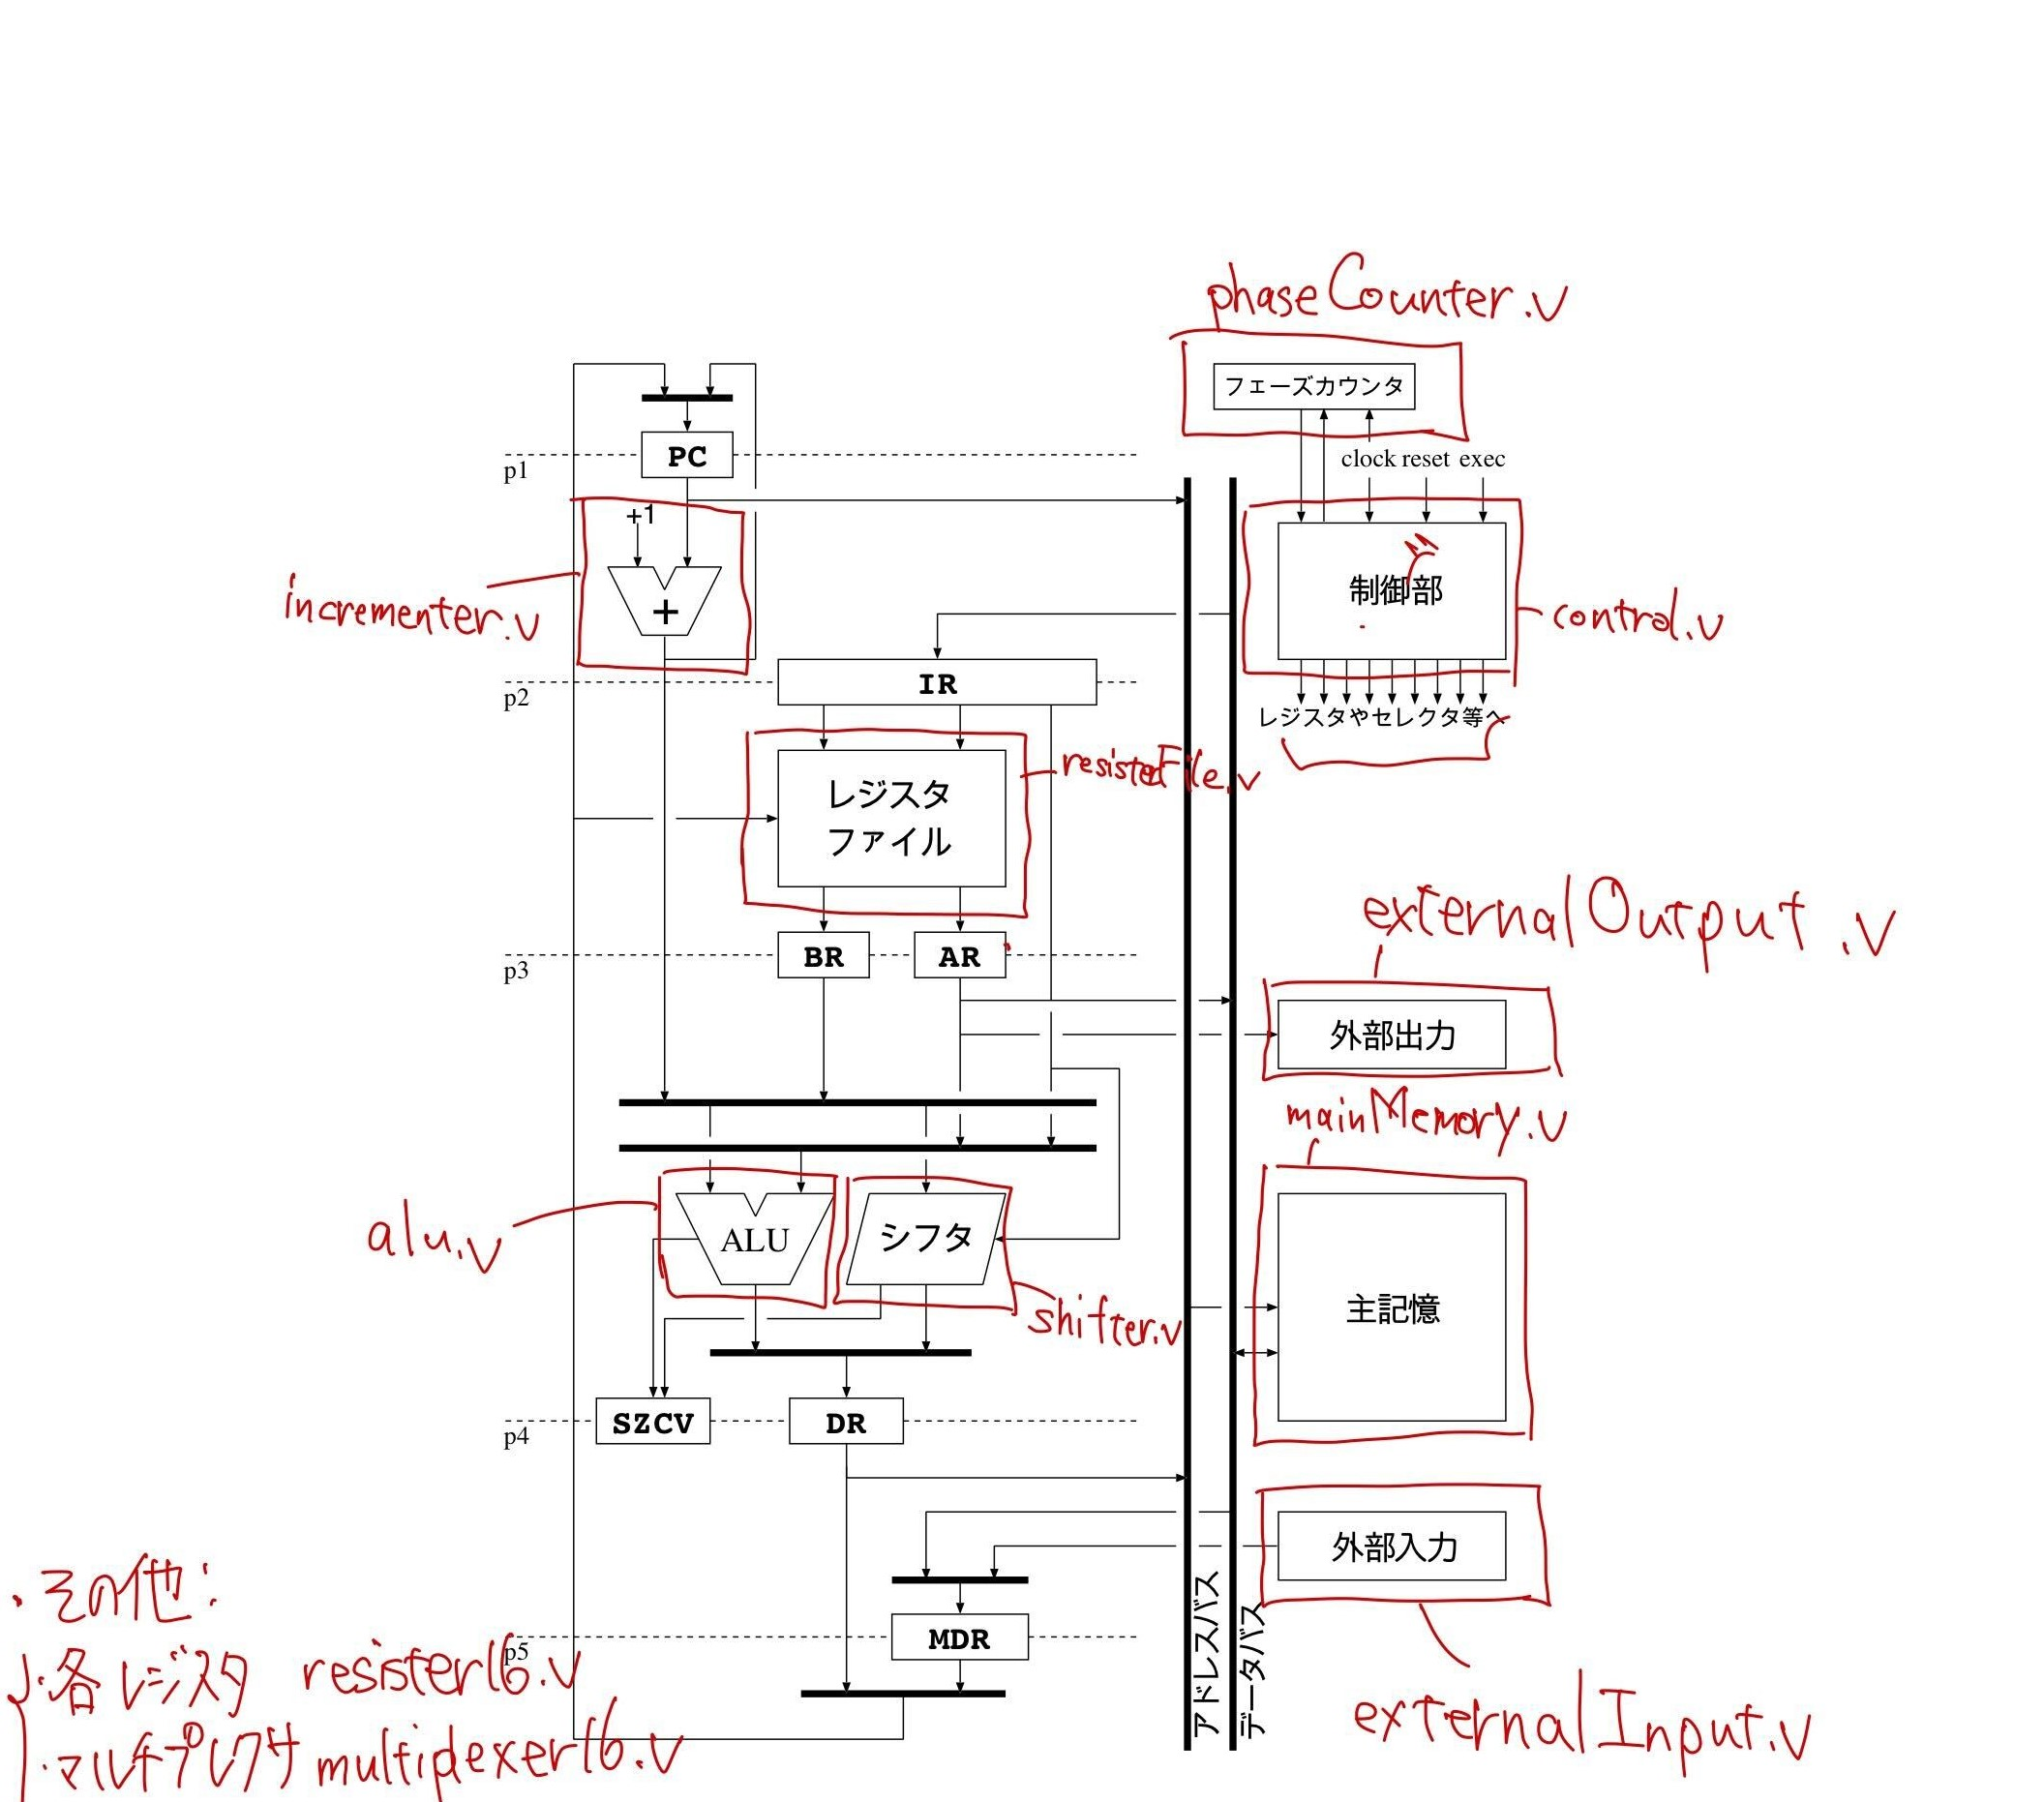
\includegraphics[scale = 0.22]{moduleSplit0422.jpg}
    \end{center}
    \caption{シミュレーションの結果続き、上段からa[3:0]、out[7:0]、seletorを表す。}
    \label{moduleSplit0422}
\end{figure}

\section{役割分担}

役割分担の表を以下の図\ref{rolesDivision0422}に示す。
その他のmultiplexer16.v,resister16.vについてはそこまで大きな回路ではないので、分担をしていない。



\begin{figure}[H]
    \begin{center}
        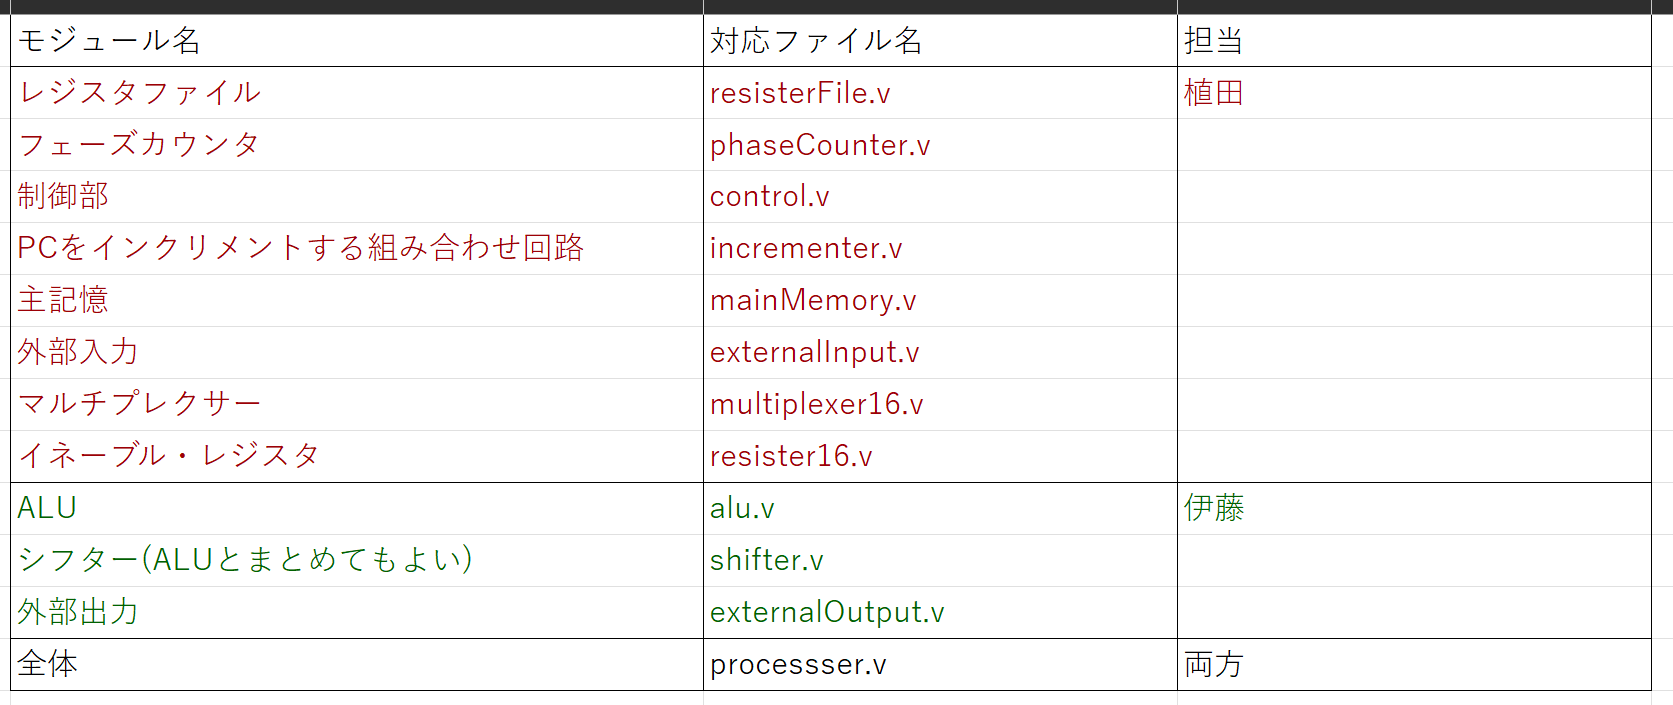
\includegraphics[scale = 0.5]{rolesDivision0422.png}
    \end{center}
    \caption{役割分担(4月22日時点)}
    \label{rolesDivision0422}
\end{figure}

\section{最終課題に対する現在の進捗状況}

\section{今後の進捗計画}



\end{document}